\documentclass[10pt]{article}
\usepackage{amsmath,graphicx}
%\usepackage[cmex10]{amsmath}
\usepackage{amssymb}
\usepackage{amsthm}
\usepackage{geometry}
\usepackage{graphicx}
\usepackage{epstopdf}
\usepackage{hyperref}
\usepackage{amsmath}
\usepackage{amssymb}
\usepackage{amsthm}
\usepackage{amscd}
\usepackage{amsfonts}
\usepackage{graphicx}%
\usepackage{fancyhdr}

% Example definitions.
% --------------------
\def\x{{\mathbf x}}
\def\L{{\cal L}}

\newcommand {\MEL} {{\mathrm{M}}}
\newcommand {\R} {{\mathbb{R}}}
\newcommand {\Z} {{\mathbb{Z}}}
\newcommand {\E} {{\mathbb{E}}}
\newcommand {\om} {{\omega}}
\newcommand {\la} {{\lambda}}
\newcommand {\La} {{\Lambda}}
\newcommand{\hS}{\widehat S}
\newcommand {\ga} {{\gamma}}
\newcommand {\ld} {{\bf l^2}}
\newcommand {\MFSC} {{\rm MFSC}}
\newcommand {\oS} {{\overline S}}
\newcommand {\lau} {{\lambda_1}}
\newcommand {\lad} {{\lambda_2}}
\newcommand {\lam} {{\lambda_m}}
\newcommand {\Omu} {{\Omega_1}}
\newcommand {\Omd} {{\Omega_2}}
\newcommand {\Omm} {{\Omega_m}}
\newcommand {\omu} {{\omega_1}}
\newcommand {\omd} {{\omega_2}}
\newcommand {\omm} {{\omega_m}}
\newcommand {\quef} {{q}}
\newcommand {\quefu} {{q_1}}
\newcommand {\quefd} {{q_2}}
\newcommand {\lat} {{\lambda_3}}
\newcommand {\cP} {{\cal P}}
\newcommand {\cPP} {{\cal P}}
\newcommand {\bV} {{\bf V}}
\newcommand {\C} {{\mathbb C}}
\newcommand {\N} {{\mathbb N}}
\newcommand {\mm} {{l}}
\newcommand {\tS} {{\widetilde{S}}}
\newcommand {\Ufreq} {{U^{\mathrm{fr}}}}
\newcommand {\Sfreq} {{S^{\mathrm{fr}}}}
\newcommand {\freq} {{{\mathrm{fr}}}}
\newcommand{\eqdist}{\stackrel{d}{=}}
\newcommand{\Exp}[1]{\mathbf{E}\left(#1 \right)}
\newcommand{\var}[1]{\text{var}\left(#1 \right)}

\newtheorem{theorem}{Theorem}[section]
\newtheorem{lemma}[theorem]{Lemma}
\newtheorem{corollary}[theorem]{Corollary}
\newtheorem{conjecture}[theorem]{Conjecture}
\newtheorem{proposition}[theorem]{Proposition}
\newtheorem{definition}[theorem]{Definition}
\newtheorem{remark}[theorem]{Remark}
\newtheorem{df}{Definition}

%\title{Research Statement}
%%\date{June 30th, 2015}
%\author{Joan Bruna}

%\oddsidemargin  0.02in \evensidemargin 0.02in

\makeatletter
\newlength{\bibhang}
\setlength{\bibhang}{1em}
\newlength{\bibsep}
 {\@listi \global\bibsep\itemsep \global\advance\bibsep by\parsep}
\newenvironment{bibsection}%
        {\vspace{0.1in}\begin{list}{}{%
       \setlength{\leftmargin}{\bibhang}%
       \setlength{\itemindent}{-\leftmargin}%
       \setlength{\itemsep}{\bibsep}%
       \setlength{\parsep}{\z@}%
        \setlength{\partopsep}{10pt}%
        \setlength{\topsep}{10pt}}}
        {\end{list}\vspace{-.6\baselineskip}}
\makeatother

\pagestyle{fancy}\lhead{Research Proposal} \rhead{September 2016}
\chead{{\large{\bf Joan Bruna}}} \lfoot{} \rfoot{\bf \thepage} \cfoot{}

\newcounter{list}

\renewcommand{\baselinestretch}{0.98}
\begin{document}
%\maketitle
%\tableofcontents


\section*{Overview}
\begin{itemize}
\item \textbf{Title:} Understanding and exploiting the loss surface of Deep Neural Networks  
\item \textbf{Principal Investigator: } Joan Bruna Estrach. Courant Institute, NYU, Computer Science Department, Mathematics Department and Center for Data Science. Contact: bruna@cims.nyu.edu; cell: 917-767-0617. 
\item \textbf{Google Sponsors:} Jascha Sohl-Dickstein, Koray Kavukcuoglu.
\item \textbf{Google Contacts:} Oriol Vinyals, Vincent Vanhoucke, Jonathan Tomson.
\end{itemize}

\section*{Proposal Body}

%\subsection{Abstract}
\textbf{Abstract:}
Training Deep Neural networks is a prime example of a high-dimensional non-convex 
optimization problem. Despite its massive practical interest, there exist little theoretical 
guarantees that can inform the choice of the training hyperparameters as well as model 
arquitectural choices. In this proposal we will study conditions 
on the data distribution and model architecture that prevent the existence 
of poor local minima, by first focusing on statistical properties of natural images
and specific convolutional architectures.
 
The conditioning of gradient descent is the next challenge we shall address. 
We study this question by estimating the geometry of the level sets of any given
loss. For that purpose, 
we introduce an algorithm to estimate the regularity of such sets on large-scale networks. 
Our initial results suggest that these sets become exponentially more curvy 
as the energy level decays, in accordance to what is observed in practice. 
A byproduct of our analysis is the development of learning algorithms that can adapt 
to the geometry of these sets and provide an extra tool to streamline the training of
large models.

\vspace{0.5cm}
\noindent
\textbf{Problem Statement:}
%clear specify a problem, a well-posed question. Do not try to cover all the ground with your question. 
%current candidate specific problems:
Optimization is a critical component in Deep Learning, governing its success in different areas of computer vision, speech processing and natural language processing. The prevalent optimization strategy is Stochastic Gradient Descent, invented by Robbins and Munro in the 50s. On the one hand, the generalization of SGD is better than one could expect 
in generic, non-convex loss surfaces. On the other hand, one may wonder if this generic optimization strategy can be adapted to operate in the class of loss surfaces defined by deep neural networks. Some reasons to believe that such adaptation is possible come from the 
variety of small modifications of SGD algorithms yielding significant speedups \cite{duchi2011adaptive, hinton2012lecture, kingma2014adam}.
This raises a number of theoretical questions as to why neural network optimization does not suffer in practice from poor local minima. Likewise, it introduces opportunities to leverage training data into adapted optimization. 

%Exploration
%Topology: theoretical model. 
The loss surface of deep neural networks has recently attracted interest 
in the optimization and machine learning communities as a paradigmatic example of 
a hard, high-dimensional, non-convex problem. 
Recent work has explored models from statistical physics \cite{dauphin2014identifying}, such as spin glasses \cite{choromanska2015loss}, 
in order to understand the macroscopic properties of the system, but at the expense of strongly simplifying the nonlinear nature of the model.
In this proposal, we do not make any such assumption and study conditions 
on the data distribution and model architecture that prevent the existence 
of bad local minima. Together with 
recent results that rigorously establish that gradient descent does not 
get stuck on saddle points \cite{lee2016gradient}, our first objective will yield guarantees that gradient descent converges
to a global optimum in deep rectified networks. 

The loss surface $F(\theta)$ of a given model can be expressed in terms of its level sets $\Omega_\lambda$, which contain all parameters yielding a loss smaller or equal than the energy level $\lambda$: $\Omega_\lambda = \{ \theta ~;~F(\theta) \leq \lambda\}$. 
A first question we address concerns the topology of these level sets, i.e. under which conditions they are connected. Connected level sets imply that one can always find a descent direction at each energy level, and therefore that no poor local minima can exist. One can verify that linear neural networks (cascaded linear operators without point-wise nonlinearities), despite defining a non-convex loss $F(\theta)$, have connected level sets and therefore can be optimized globally using gradient descent strategies \cite{danieljoan}. It is also easy to verify that the non-linear case is not true in general \cite{shamir}, and our first objective is thus to characterize the interplay between data distribution, overparametrization and model architecture that is needed to obtain connected level sets \cite{danieljoan}.

%Geometry: exploring loss surface
Beyond the question of whether the loss contains poor local minima, the immediate follow-up question that determines the convergence of algorithms in practice is the local conditioning of the loss surface. It is thus related not to the topology but to the shape or geometry of the level sets. As the energy level decays, one expects the level sets to reveal more complex irregular structures, which correspond to regions where $F(\theta)$ has small curvature.

In order to construct meaningful theoretical models, we have developed an algorithm \cite{danieljoan} that efficiently estimates these topological and geometrical properties on large deep architectures and datasets. Inspired by \cite{goodfellow2014qualitatively}, given two parameter values $\theta_1$ and $\theta_2$ lying in the border of the same level set $\Omega_\lambda$, our algorithm constructs a geodesic $\gamma(t)$ in $\Omega_\lambda$ relying $\theta_1$ to $\theta_2$ using a dynamic programming procedure. An example of the resulting characteristics is illustrated in Figure 1. 

%Exploitation
\begin{figure}
\label{figurelength}
\centering
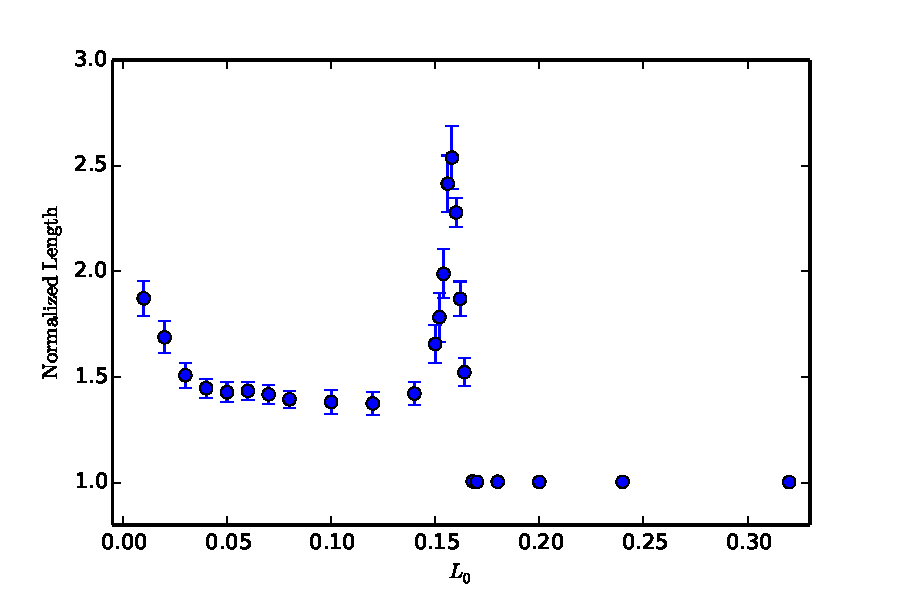
\includegraphics[width=.4\textwidth]{../Writeup/Plots/normlengthcubics}
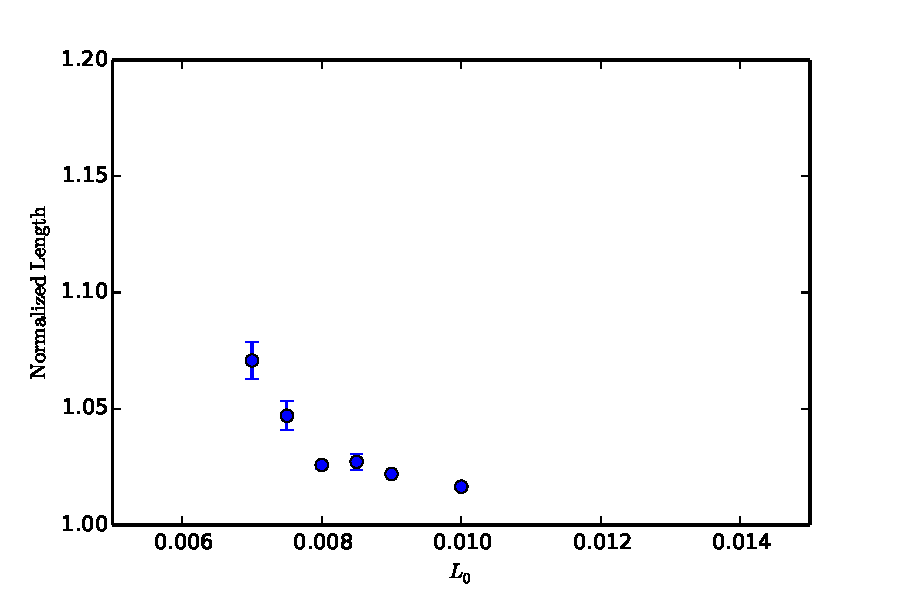
\includegraphics[width=.4\textwidth]{../Writeup/Plots/normlengthMNIST}
\caption{Normalized geodesic length as a function of the energy level for two different models. Left: a ``low-dimensional" neural network 
attempting to fit a cubic polynomial. Right: a convolutional neural network on MNIST. Whereas the cubic fitting displays a heavily non-convex structure 
at mid-energy values, the MNIST example qualitatively behaves as a convex loss, in which geodesics approach straight lines.}
\end{figure}

%Geometry: exploiting structure to optimize gradients.
Besides improving our understanding of stochastic optimization in the class of neural networks, our second main objective is to leverage that understanding 
by developing optimization strategies adapted to the class of loss surfaces at hand, i.e. learning how to learn \cite{andrychowicz2016learning}. 
In particular, we shall construct targets for optimization based on the geodesic paths described above: given two parameter values 
$\theta_a$, $\theta_b$ with $F(\theta_b) \leq F(\theta_a)=\lambda$ (for example obtained during the course of a vanilla optimization method at iterations $t$ and $t+T$ respectively), a natural target to update $\theta_a$ is to follow the geodesic $\gamma(t)$ in $\Omega_\lambda$ relying $\theta_a$ to $\theta_b$. 
The extent by which this geodesic is smooth will determine how easy it is to predict from past and present information available at $\theta_a$. We will explore predictive models based on recurrent neural networks, inspired from \cite{andrychowicz2016learning}.

\section*{Data Policy}

This proposal requires mostly unlabeled data in the form of images, speech and audio signals,
and text corpus. The initial plan is to use publicly available datasets.
The research outcomes will be both conference and journal papers, and also publicly available code. 

\section*{Budget}

\begin{itemize}
\item Student salary: \$50000 per year.
\item Student conference/workshop travel: \$6000 per year (three conferences a year). 
\end{itemize}

{\small 
\bibliographystyle{IEEEtran}
\bibliography{refs}
}

\end{document}

